\cleardoublepage
\chapter{外文翻译}

\section*{摘要}
我们呈现基于相空间体系量子动力学(SMD)的半经典磨雅动力学方法。相比于Prezhdo    等人发明的基于海森堡方程的量子化哈密顿动力学方法,SMD使用了磨雅方程来描述期望值的含时演化,并使用了辅助相空间分布的方法来对动力学方程进行截断。此时,繁琐的算符对易子的推导将不再被需要,同时能够实现任意阶的半经典含时演化。其较为优越的简洁性,灵活性以及可靠性在三个非常具有代表性,含有强烈的量子效应的模型系统中得到体现。

\section{导言}
分子动力学(MD)一直以来都作为分析动力学性质的强力工具在化学,物理,生物以及材料科学方面得到广泛应用。然而,其简单而高效的性质却又来自于对显著的量子效应(如隧穿效应,态分叉,退相干,零点能等)的描述的精度的牺牲。相比之下,量子力学方法能够提供非常精确的解释,然而却由于其复杂性及高计算成本而局限于小系统。因此,研发能够同时具有精度和效率的半经典及混合量子经典方法成为了过去几十年以来的研发重点。

在2000年,Prezhdo以及Pereverzev提出了半经典动力学方法——量子哈密顿动力学方法(QHD)。通过使用海森堡方程,该方法能够达到任意阶数的可观察量的含时演化。阶数截断能够对精确的量子力学效应提供不同程度的近似。比如,第一阶QHD(QHD-1)等价于经典的哈密顿动力学,而在添加更高阶的修正的过程中量子效应被自然而然地考虑了进去。QHD被应用于多种问题,如分子振动频率分析,亚稳态下的量子隧穿,双缝实验的干涉条纹,不同振动模式之间的能量传递,在双分子之间的振动相干转移,电子-光子耦合系统中的态跃迁,以及低温有机化合物的电荷迁移现象。QHD在多种量子问题中展现了其良好的性价比。

在QHD的基础上,一些变种也同样被发展出来。其中包括量子化平均场(QMF)方法,将系统分为全量子和半经典的两个部分,并分别用薛定谔方程和QHD方法进行描述。两个系统之间的相互作用,非绝热动力学性质通过平均场的方法进行描述。Shigeta以及其同事研发的量子累计量动力学方法在推导中充分利用了位移算符以及累计量。作为QHD方法的延伸,QCD在多种场合,如磁场下的量子修正,摩尔斯簇合物的结构优化,能够更好地实现能量守恒。最近,Smith以及Akimov提出了耦合轨迹哈密顿动力学(ETHD)方法,将一般的二阶QHD改写为耦合的经典轨迹。ETHD能够在多个测试模型下和全量子解有高度的一致性。

尽管获得了巨大的成功,QHD及其变体具有多个本质上的缺点。也就是,对动力学方程的推导要求非常繁琐的推导及其困难。尤其是Weyl对称化应被使用于位置与动量算符的交叉项,从而进一步增加了推导的复杂性。并且,为估计低阶量中的高阶量部分需要进行封闭近似,而一般的算符封闭近似却又十分难以实现。在这些文章中,平均只有前五阶的被解构的动力学算符的方程被给出,而目前只有其中的第二、三、四阶的QHD被充分利用。作为含有最低阶的量子修正,QHD-2在过去的研究中最受欢迎。事实上,QHD-2能够通过对维数进行倍增和经典力学一一对应,并和解冻高斯波包动力学有高度的相关性。总体而言,对量子动力学的精确描述需要更高阶的半经典解进行描述,而其并未得到充分研究。

在本文章中,我们提出一个具有创新意义的半经典磨雅动力学(SMD)框架来对任意阶的半经典动力学进行一个一般的描述。在相空间体系下,我们推导一般性的动力学演化方程并引入辅助相空间分布方法,其提供了一般的耦合动力学方程的闭合近似方法。作为示例,SMD被应用于(1)亚稳定的三次项势能的衰变动力学,(2)在摩尔斯势下的振动以及(3)双势阱势能下的势垒穿越。

\section{理论}
\subsection{量子力学的相空间表述}
在一个具有总哈密顿量$\hat{H}$的体系中,任意可观察量$\hat{A}$的含时演化遵从海森堡方程
\begin{equation}
	\frac{d}{d t} \hat{A}_{H}=\left(\frac{\partial \hat{A}}{\partial t}\right)_{H}+\frac{1}{i \hbar}\left[\hat{A}_{H}, \hat{H}\right]
\end{equation}
其中下标$H$表示在海森堡绘景下的算符,$\hbar$为标化普朗克常数,以及 $[\cdot,\cdot]$表达两个算符的对易子。将两边取期望值,得到
 \begin{equation}
	\frac{d}{d t}\langle\hat{A}\rangle=\left\langle\frac{\partial \hat{A}}{\partial t}\right\rangle+\frac{1}{i \hbar}\langle[\hat{A}, \hat{H}]\rangle
	\label{Heisenberg}
\end{equation}
从希尔波特空间表象切换至等价的相空间表象得到磨雅动力学方程
\begin{equation}
	\frac{d}{d t}\langle A\rangle=\left\langle\frac{\partial A}{\partial t}\right\rangle+\langle\{\{A, H\}\}\rangle
	\label{Ehrenfest}
\end{equation}
其中$A$ 和$H$ 分别代表坐标和动量的实函数,并为量子力学算符$\hat{A}$ 和$\hat{H}$ 在相空间下的等价表述。$\langle A \rangle $ 为$A$ 在相空间分布下的平均值,并取代$\langle \hat{A} \rangle $ 描述期望值。$\{\{\cdot, \cdot\}\}$为磨雅括号,定义为
 \begin{equation}
	 \{\{f, g\}\}=\frac{2}{\hbar} f \sin \left[\frac{\hbar}{2}\left(\sum_{i} \overleftarrow{\partial}_{q_{i}} \overrightarrow{\partial}_{p_{i}}-\overleftarrow{\partial}_{p_{i}} \overrightarrow{\partial}_{q_{i}}\right)\right] g
\end{equation}
其中$f$和 $g$ 为相空间函数,指标$i$遍历所有坐标$\{q_i\}$和动量$\{p_i\}$ 下的自由 度,而左箭头和右箭头分别代表向左和向右的偏微分。

为了简洁而又不失一般性,我们将哈密顿量视为只有一个自由度,
\begin{equation}
	H=\frac{p^{2}}{2 m}+V(q)
	\label{Hamiltonian}
\end{equation}
其中$m$ 为粒子的质量。将(\ref{Hamiltonian})代入(\ref{Ehrenfest}),得到
\begin{equation}
	\frac{d}{d t}\langle A\rangle=\left\langle\frac{\partial A}{\partial t}\right\rangle+\langle\{A, H\}\rangle+\sum_{k=1}^{\infty} \frac{(-1)^{k+1} \hbar^{2 k}}{(2 k+1) ! 2^{2 k}}\left\langle A_{p}^{(2 k+1)} V_{q}^{(2 k+1)}\right\rangle
	\label{Moyalgeneral}
\end{equation}
其中我们使用了缩写$A_{p}^{(i)}=\partial^{i} A / \partial p^{i}$以及 $V_{q}^{(i)}=\partial^{i} V / \partial q^{i}$.泊松括号被定义为
\begin{equation}
	\{f, g\}=\frac{\partial f}{\partial q} \frac{\partial g}{\partial p}-\frac{\partial f}{\partial p} \frac{\partial g}{\partial q}
\end{equation}
显然,$\hbar$只在右手边第三项出现,且仅当对应的$A$和 $V$项的偏导存在时非零 。

\subsection{相空间下的耦合方程的期望值}
将(\ref{Moyalgeneral})中的$A$取代为不同的相空间变量得到一阶的不同含时演化方程。比如,将 $A$设为 $q$或 $p$,得到
\begin{equation}
\frac{d}{d t}\langle q\rangle=\frac{1}{m}\langle p\rangle
\label{Ehrenfestq}
\end{equation}
\begin{equation}
\frac{d}{d t}\langle p\rangle=-\left\langle V_{q}^{(1)}\right\rangle	
\end{equation}
即众所周知的艾伦非斯特方程。值得注意的是相似的方程也能从(\ref{Heisenberg})基于相对应的算符的期望值推得。为得到在封闭的方程系统,我们一般需要继续得到$\langle V_q^{(1)} \rangle $ 对时间的偏导,
\begin{equation}
	\frac{d}{d t}\left\langle V_{q}^{(1)}\right\rangle=\frac{1}{m}\left\langle V_{q}^{(2)} p\right\rangle
\end{equation}
其依赖于高阶项$\langle V_q^{(2)} p \rangle $.其对应方程为
\begin{equation}
	\frac{d}{d t}\left\langle V_{q}^{(2)} p\right\rangle=\frac{\left\langle V_{q}^{(3)} p^{2}\right\rangle}{m}-\left\langle V_{q}^{(1)} V_{q}^{(2)}\right\rangle
\label{EhrenfestV2}
\end{equation}
这些对时间的偏导的推导可一直重复,且总体而言,会导致无穷数量的耦合动力学方程。值得一提的是在方程(\ref{Ehrenfestq})-(\ref{EhrenfestV2})和Akimov及Prezhdo直接得到的变量有一定的联系。

为得到更一般的动力学方程的表达式,我们假设势能面可以被估计为$M$阶多项式
\begin{equation}
	\frac{d}{d t}\left\langle V_{q}^{(2)} p\right\rangle=\frac{\left\langle V_{q}^{(3)} p^{2}\right\rangle}{m}-\left\langle V_{q}^{(1)} V_{q}^{(2)}\right\rangle
\label{Polypotential} 
\end{equation}
其中$a_k$ 为各项系数。这可以通过对势能面在固定的某一点或一直移动的一点上进行展开。在实际计算中,有些体系可能需要相当大的$M$才能得到较为让人满意的结果。即便如此,我们仍旧假设体系势能 能够被表达为多项式并展开对我们的方法的叙述。显然,在(\ref{Ehrenfestq})-(\ref{EhrenfestV2})各方程中变量变为不同阶的$q^ip^j$的线性组合。第一阶变量为 $q$及 $p$,其动力学方程由(\ref{Ehrenfestq})及(\ref{Ehrenfestq}+1)两式得到。对于第二阶项(即 $q^2,\,qp,$ 以及$p^2$),将(\ref{Polypotential})代入(\ref{Moyalgeneral})得到
\begin{equation}
\frac{d}{d t}\left\langle q^{2}\right\rangle=\frac{2}{m}\langle q p\rangle
\end{equation}
\begin{equation}
	\frac{d}{d t}\langle q p\rangle=\frac{\left\langle p^{2}\right\rangle}{m}-\sum_{k=1}^{M} k a_{k}\left\langle q^{k}\right\rangle
	\label{Ehrenfestqp}
\end{equation}
\begin{equation}
	\frac{d}{d t}\left\langle p^{2}\right\rangle=- 2 \sum_{k=1}^{M} k a_{k}\left\langle q^{k-1} p\right\rangle
	\label{EhrenfestP2}
\end{equation}
总体上,$N$阶项的动力学演化方程中会出现 $N+1$阶项。从(\ref{Ehrenfestqp})及(\ref{EhrenfestP2})二式来看,当$M>2$时二阶项的期望值依赖于更高阶的项。结论同样适用于高于二阶的项。

不同的相空间变量组能够用来建立耦合的动力学方程。Prezhdo展现了即时的坐标及动量的平均值可以推出简化的动力学方程。同样地,我们选择 $\mu_q=\langle q \rangle $,\,$\mu_p = \langle p \rangle $,\,$\sigma_q = \sqrt{\langle (q-\mu_q)^2 \rangle }$, 以及$\sigma_p = \sqrt{\langle (p-\mu_p)^2 \rangle }$并定义不含单位的坐标及动量 $\tilde{q}=\left(q-\mu_{q}\right) / \sigma_{q}$以及 $\tilde{p}=\left(p-\mu_{p}\right) / \sigma_{p}$,这样能够使数值计算更为方便。那么 $\tilde{q}^{i} \tilde{p}^{j}$可替代 $q^{i} p^{j}$.其期望值,$\xi_{i j}=\left\langle\tilde{q}^{i} \tilde{p}^{j}\right\rangle$,具有性质 $\xi_{00}=1, \xi_{10}=\xi_{01}=0$,以及 $\xi_{20}=\xi_{02}=1$.从式(\ref{Polypotential})我们可以用$\tilde{q}$的多项式表达 $V$ 
\begin{equation}
	V(\tilde{q})=\sum_{k=0}^{M} b_{k} \tilde{q}^{k}
\end{equation}
令$b_{k}=\sum_{l=k}^{M} C_{l}^{k} \mu_{q}^{l-k} \sigma_{q}^{k} a_{l}$以及 $C_{m}^{n}=m ! /[n !(m-n) !]$.将上式应用到式(\ref{Moyalgeneral})得到完整的一系列耦合动力学方程
\begin{equation}
	\frac{d}{d t} \mu_{q}=\frac{\mu_{p}}{m}
	\label{muq}
\end{equation}
\begin{equation}
	\frac{d}{d t} \mu_{q}=\frac{\mu_{p}}{m}
\end{equation}
\begin{equation}
	\frac{d}{d t} \sigma_{q}=\frac{\sigma_{p} \xi_{11}}{m}
\end{equation}
\begin{equation}
	\frac{d}{d t} \sigma_{p}=\chi
\end{equation}
\begin{equation}
	\begin{aligned} \frac{d}{d t} \xi_{i j}=& \alpha \xi_{i j}+\beta \xi_{i-1, j+1}+\gamma \xi_{i, j-1} \\ &+\sum_{k=0}^{K} \sum_{j=1}^{M} \eta_{k l} \xi_{i-2 k-1+l+l, j-2 k-1} \end{aligned}
	\label{dimensionless}
\end{equation}
其中我们引入了符号
\begin{equation*}
	\begin{cases}
	\alpha=-j \chi / \sigma_{p}-i \xi_{11} \sigma_{p} / (m\sigma_q),\\
	\beta=i \sigma_{p} /\left(m \sigma_{q}\right),\\
	 \gamma=-j \lambda / \sigma_{p}, \\
	 \eta_{k l}=(-1)^{k+1} b_{l}\hbar^{2 k} C_{j}^{2 k+1} A_{l}^{2 k+1} /\left(2^{2 k} \sigma_{p}^{2 k+1} \sigma_{q}^{2 k+1}\right),\\
	 \lambda=-\sum_{k=1}^{M} k b_{k} \xi_{k-1,0} / \sigma_{q}, \\
	 \chi=-\sum_{k=1}^{M} k b_{k} \xi_{k-1,1} / \sigma_{q} 
	\end{cases}
\end{equation*}
以及$A_{m}^{n}=m ! /(m-n) !$来对公式进行简化,而 $K$为不大于 $(\min \{j, M\}-1) / 2$的最大整数。从公式(\ref{dimensionless}),我们可以看出任意$i+j$阶变量$\xi_{ij}$ 依赖于变量$\xi_{kl}$,其最高阶项为 $i+j+M-2$.

\subsection{动力学方程截断}
对$M>2$的势能多项式,无穷数量的耦合动力学方程需要通过使用低阶量对高阶量进行拟合来截断。在本文中,我们使用(\ref{muq})-(\ref{dimensionless})得到前$N$阶的含时演化方程,并使用$P_N(q,p)$进行截断。我们的方法为利用低阶量获得$P_N(q,p)$的表达式,并利用该表达式计算估计的高阶量。一般地,我们可以将$P_N(q,p)$表达为基组的线性展开
\begin{equation}
	P_{N}(q, p)=\sum_{0 \leq k+l \leq N} c_{k l} f_{k l}(q, p)
	\label{basis_expansion}
\end{equation}
其中$\left\{f_{k l}(q, p)\right\}$为基组函数,$\{c_{kl}\}$为每项对应系数。于是对没一项$\xi_{ij}$,我们能够得到以下方程
\begin{equation}
	\xi_{i j}=\sum_{0 \leq k+l \leq N} M_{i j, k l} c_{k l}
	\label{xi_ij}
\end{equation}
其中$M_{i j, k l}=\int f_{k l}(q, p) \tilde{q}^{i} \tilde{p}^{j} d q d p$.对第$N$阶的SMD(SMD-$N$),对$0 \leq i+j \leq N$的$\xi_{ij}$已知,而从公式(\ref{xi_ij})能得到的线性方程组数量为$(N+1)(N+2)/2$,正好等于公式(\ref{basis_expansion})中系数的数量。此时我们可以利用公式(\ref{xi_ij})得到的系数组推得$i+j>N$的$\xi_{ij}$项并得到$i+j\leq N$的$\xi_{ij}$项的含时演化。

公式(\ref{basis_expansion})中的基组函数可选择不同形式。利用从简谐振子的特征解获得的灵感,我们使用高斯基组
\begin{equation}
	f_{k l}(q, p)=f(q, p) \tilde{q}^{k} \tilde{p}^{l}
	\label{dimenstionless_phasespace}
\end{equation}
其中
\begin{equation*}
f(q, p)=\frac{\exp \left\{-\frac{\left(q-\mu_{q}\right)^{2} / \sigma_{q}^{2}-2 \rho\left(q-\mu_{q}\right)\left(p-\mu_{p}\right)/\left.\left.\left(\sigma_{q} \sigma_{p}\right)+\left(p-\mu_{p}\right)^{2} / \sigma_{p}^{2}}{2\left(1-\rho^{2}\right)}\right\}}{2 \pi \sigma_{q} \sigma_{p}\left(1-\rho^{2}\right)^{1 / 2}}
\end{equation*}
为相关系数为$\rho = \xi_{11}$的标准双变量正态分布。那么公式(\ref{xi_ij})中的矩阵元变为$M_{i j, k l}=\int f(q, p) \tilde{q}^{i+k} \tilde{p}^{j+l} d q d p$,而其可基于Wick定理进行计算,即若$i+j+k+l$为奇数,$M_{ij,kl}$永远为零;否则,我们有
\begin{equation}
	M_{i j, k l}=\sum_{n=0}^{I} \rho^{a-2 n} C_{a}^{2 n} A_{b}^{a-2 n}(2 n-1) ! !(b-a+2 n-1) ! !
	\label{matrixelement}
\end{equation}
该式只依赖于$a = \min \{i + k, j + l\}$及$b = \max \{i+k, j+l\}$. $I$为不超过$a/2$的最大整数。由此我们可以将$(N+1)(N+2)/2$个线性方程组分解为两个子系统:一个具有奇数的$i+j$和$k+l$,另一个具有偶数的$i+j$和$k+l$.

\subsection{SMD的流程}
作为实例,我们使用具有$M$阶多项式势能的一维体系阐述我们的半经典动力学$N$阶SMD流程:
\begin{enumerate}
	\item 在零时刻,我们根据我们研究的问题设定波函数$\psi(q)$,并由此推出初始变量(如$\mu_q$, $\mu_p$, $\sigma_q$, $\sigma_p$, $\rho$, 和$3\leq i+j \leq N$的$\{\xi_{ij}\}$ 项)。若为高斯波包,
	\begin{equation}
		\psi(q)=\left(\frac{m \omega}{\pi \hbar}\right)^{1 / 4} \exp \left[-\frac{m \omega\left(q-q_{0}\right)^{2}}{2 \hbar}+i \frac{p_{0} q}{\hbar}\right]
	\end{equation}
	利用维格纳变换,我们得到对应的相空间分布
	\begin{equation*}
	P(q,p) = \exp \left\{-\left[\left(q-\mu_{q}\right)^{2} /\left(2 \sigma_{q}^{2}\right)+\left(p-\mu_{p}\right)^{2} /\left(2 \sigma_{p}^{2}\right)\right]\right\} / (2\pi \sigma_q \sigma_p).
	\end{equation*}
	 此时,我们可以轻易地计算相空间期望值$\mu_{q}=q_{0}, \,\mu_{p}=p_{0},\, \sigma_{q}=\sqrt{\hbar /(2 m \omega)},\,$ $\rho=0,\,$以及$\sigma_p = \sqrt{m\hbar \omega /2 }$. 若$i$和$j$同时为偶数,$\xi_{ij} = (i-1)!!(j-1)!!$; 否则在$t=0$时$\xi_{ij} = 0$.
	\item 在每个$t$时刻,我们利用四阶隆格-库塔法计算经过$dt$时间间隔后的SMD的各变量。此时,我们先计算矩阵$M_{i j, k l}$.对公式(\ref{dimenstionless_phasespace})中的基组函数,若$i+j+k+l$为偶数则$M_{ij,kl}$满足公式(\ref{matrixelement}),否则为零。利用公式(\ref{xi_ij})所提供的$0\leq i + j \leq N$的线性方程,我们得到$\{c_{kl}\}$以及相应的辅助相空间分布,$P_N(q,p)$.而后我们利用公式(\ref{xi_ij})计算$N+1\leq i+j \leq N+M-2$ 下的 $\{\xi_ij\}$的值并接入公式(\ref{muq})-(\ref{dimensionless})中的等式右边得到完整的微分方程。该步骤一直重复至满足某一个先决条件。
	\item 对任意一个可观察量$A(p,q)$,其期望值的含时演化通过含时辅助相空间分布计算得到:
	\begin{equation}
		\langle A(p, q, t)\rangle=\int A(p, q) P_{N}(x, p, t) d q d p
	\end{equation}
	由此,我们便得到了一个完整的建立在有限数量的期望值的半经典动力学方法。
\end{enumerate}
\subsection{QHD与SMD之间的关系}
与QHD-1相似,SMD-1提供了经典力学体系下的哈密顿方程(见附录A)。对SMD-2,方程(\ref{xi_ij})转化为一个奇数和偶数的线性方程子系统:
\begin{equation}
	\left[\begin{array}{ll}
{1} & {\rho} \\
{\rho} & {1}
\end{array}\right]\left[\begin{array}{l}
{c_{10}} \\
{c_{01}}
\end{array}\right]=\left[\begin{array}{l}
{0} \\
{0}
\end{array}\right]
\end{equation}
以及
\begin{equation}
	\left[\begin{array}{cccc}
{1} & {1} & {1} & {\rho} \\
{1} & {3} & {1+2 \rho^{2}} & {3 \rho} \\
{1} & {1+2 \rho^{2}} & {3} & {3 \rho} \\
{\rho} & {3 \rho} & {3 \rho} & {1+2 \rho^{2}}
\end{array}\right]\left[\begin{array}{l}
{c_{00}} \\
{c_{20}} \\
{c_{02}} \\
{c_{11}}
\end{array}\right]=\left[\begin{array}{c}
{1} \\
{1} \\
{1} \\
{\rho}
\end{array}\right]
\end{equation}
其解为$c_{00} = 1$ 和 $c_{10}=c_{01}=c_{20}=c_{02}=c_{11}=0$, 从而给出和二阶QCD相同的相空间分布。从方程(\ref{xi_ij}),SMD截断变为$\xi_{i j} \approx M_{i j, 00}$. 此时,$\xi_{04}=\xi_{40} \approx 3, \xi_{22} \approx 1+2 \rho^{2}$,以及$\xi_{13}=\xi_{31} \approx 3 \rho$, 同时所有第三阶和第五阶期望值为零。相比之下,QHD的截断方法同样保证了第三阶和第五阶的$\left\langle\tilde{q}^{i} \tilde{p}^{j}\right\rangle$在QHD中被估计为$\left\langle\tilde{p}^{4}\right\rangle \approx 3\left\langle\tilde{p}^{2}\right\rangle\left\langle\tilde{p}^{2}\right\rangle= 3$, $\left\langle\tilde{q}^{4}\right\rangle \approx 3\left\langle\tilde{q}^{2}\right\rangle\left\langle\tilde{q}^{2}\right\rangle= 3$, $\left\langle\tilde{q}^{2} \tilde{p}^{2}\right\rangle \approx\left\langle\tilde{q}^{2}\right\rangle\left\langle\tilde{p}^{2}\right\rangle+ 2\langle\tilde{q} \tilde{p}\rangle\langle\tilde{q} \tilde{p}\rangle= 1+2 \rho^{2}$, $\left\langle\tilde{q} \tilde{p}^{3}\right\rangle \approx 3\langle\tilde{q} \tilde{p}\rangle\left\langle\tilde{p}^{2}\right\rangle = 3 \rho$, 以及$\left\langle\tilde{q}^{3} \tilde{p}\right\rangle \approx 3\left\langle\tilde{q}^{2}\right\rangle\langle\tilde{q} \tilde{p}\rangle= 3 \rho$,这和我们的在相空间得到的结果相一致。事实上,我们仔细验证了SMD-3和SMD-4中的所有低于五阶的截断方程。我们利用(\ref{basis_expansion})和(\ref{dimenstionless_phasespace})得到的截断方法一直都和Prezhdo提出的QHD截断结果相一致。值得一提的是更高阶的QHD截断由于非常复杂的化简公式没有给出(见附录B),而在相空间体系下任意阶的截断方程可利用上述公式轻松实现。因此,现有的SMD方法能够提供量子化的哈密顿动力学的精确描述。

\section{结果与讨论}
SMD方法被应用于研究三个一维模型体系,各自采用不同的势能面:(A)三次方势能,(B)摩尔斯势,(C)双势阱。A模型为在文献中被深入研究的系统,其中量子隧穿效应起到了很重要的作用。在这里,我们使用该模型来将我们的SMD方法和QHD的结果进行对比。模型B与C为更为复杂的系统,我们通过对高于五阶的变量进行截断来得到对动力学更好的描述。在这两个模型中,SMD的结果与精确的量子动力学结果DVR方法进行了比较。DVR的时间间隔被选定为哈密顿矩阵的光谱半径的倒数。在以下计算中,若另未声明皆使用原子单位制。

\subsection{亚稳态三阶势能下的衰变}
我们研究的第一个模型为三阶势能,
\begin{equation}
	V(q)=q^{2} / 2+q^{3} / 6
\end{equation}
该模型模拟了电子从一个亚稳态以隧穿形式脱离的过程。质量被设定为1.在$q=0$附近,势能能够被近似描述为简谐势能$V(q)=q^2/2$,其对应的基态被用来作为初始波函数,
\begin{equation}
	\psi(q)=\pi^{-1 / 4} \exp \left(-q^{2} / 2\right)
\end{equation}
势能面和初始实空间分布展现于图 (1(a)).该亚稳态被设计为只能通过隧穿的形式脱离。该模型曾被Prezhdo和Pahl系统研究过。研究证明将截断阶数从二阶提升至四阶能够显著提升QHD的精度。在图 (1(b))中,我们展现了SMD的数值结果。我们使用0.1 a.u.的时间元来得到收敛的结果。其截断基于方程(22)与(24)所述辅助相空间分布得到。显然,SMD的截断方式能够给出和同阶的QHD完全相同的结果。


\subsection{摩尔斯势能下的振动}
第二个模型为摩尔斯势能(见图 (2(a))),
\begin{equation}
	\psi(q)=\pi^{-1 / 4} \exp \left(-q^{2} / 2\right)
\end{equation}
其中$a=4.419 \, \mathrm{eV},\, b = 2.567 \AA ^{-1}$, 以及 $m=1836$.其被设计为描述在水分子中氧和氢的非简谐振动。与A模型相似,初始波函数被设定为在势能最低点处的近似简谐势能对应的基态。为处理这样的非多项式势能,我们利用了Prezhdo和Pereverzev提出的固定框架近似,即我们将摩尔斯势进行泰勒展开,
\begin{equation}
	V(q) \approx \sum_{n=0}^{M} \frac{1}{n !} V_{q}^{(n)}(0) q^{n}
\end{equation}
其中$V_{q}^{(n)}$ 为势能关于坐标的$n$阶导。使用更高数值的$M$能够得到更好的结果。

在图 (2(b))和(2(c))中,我们展现了SMD-2的平均位移和平均动量的含时演化。相比于模型A,更大的质量允许我们使用更长的时间元$dt=10\,\mathrm{a.u.}$进行动力学模拟。作为对比,DVR的结果使用了范围为$[-0.76,2.00]$,间隔为0.01的格点。我们可以发现增大$M$能够显著提升精度。$M=6$下的SMD-2能够或多或少提供收敛于DVR的结果。我们知道在$SMD-N$中势能最高阶$M$下的最高无单位变量截断为$N+M-2$。因此,在这里最高阶截断为第六阶,超过了在文献中使用的五阶截断。相比之下,现有的SMD方法能够得到令人满意的动力学模拟结果。在图(2(b))和(2(c))中,我们同时展现了经典MD的结果。由于我们初始条件的选择,粒子被固定在了原点。因此,该动力学演化完全是量子效应的结果。

\subsection{双势阱下的势垒穿越}
在第三个模型中,我们考虑一个对称的双陷阱势能(见图(3(a)))
\begin{equation}
	V(q)=a q^{2}+b q^{4}
\end{equation}
其中$a=-3 \times 10^{-4}, b=2.4 \times 10^{-5}, \text { 以及 } m=1836$.设计初衷为势垒高度约为$k_B T$,其中$k_B$为玻尔兹曼常数,$T$为室温。两个局部最小值的距离为$5 \, \mathrm{a.u.}$,是非常典型的分子间距离。初始波函数被选定为在左边的势阱最低点
\begin{equation}
	\psi(q)=(2 \pi d)^{-1 / 4} \exp \left[-\left(q-q_{0}\right)^{2} /(4 d)+i p_{0} q\right]
\end{equation}
其中$d=0.25$, $q_0=-2.5$,以及$p_0=2$.在DVR计算中,我们考虑一个在$[-10,10]$范围内,0.05为间隔的格点。在图(3(b))中,我们研究了在$dt=10 \, \mathrm{a.u.}$下的相空间轨迹。SMD阶数的增多能够促进系统级的轨迹的收敛性的提升,同时SMD-10能够定量复现DVR的结果。在该模型中,最高的变量截断为12阶,而该截断在希尔波特空间中很难实现。相比之下,经典的MD结果与量子力学体系下的结果截然不同。为了更好地对SMD进行评估,我们同时研究了二阶变量的含时演化(见图(4))。再一次地,SMD的结果在所有情况下通过提高阶数能系统性地收敛于量子精确解。

最后,我们指出SMD提供了一个研究半经典动力学的非常灵活的理论框架。在现有的研究中,我们使用了无单位的变量,辅助相空间分布的线性展开,以及一个高斯型函数基组来测试SMD的能力。在这些选择下的低阶SMD能够浮现传统QHD的结果。然而SMD的框架能够对调整含时演化的变量组和帮助截断的辅助相空间分布提供非常大的灵活性。因此,SMD在处理复杂动力学问题时具有超过已有的以期望值为基础的方法的能力。同时,我们使用一维多项式是能作为例子来展现SMD的流程。广义上的势能同样可以按照类似的方法进行研究。随着维度的增多计算成本可能会由于更多的变量而显著增加,因此需要开发更为高效的流程。初始构型同样可能对动力学具有重大影响。如果考虑热力学系统,可以对简谐振子使用简单的量子初始条件。相关研究仍在进行中。

\section{结论}
作为总结,我们将传统的QHD方法衍生到了相空间系统。对应的半经典SMD方法在简洁性,一般性以及灵活性上显示出了巨大的优势。为推导动力学方程而必需的繁琐的Weyl对称化以及算符代数不再被需要,同时SMD提供了一个系统的变量截断方法。我们采用了一系列变量以及辅助相空间分布来刻画SMD的能力。通过三个模型系统作为示例,我们展现了低阶SMD能够复现QHD的结果,同时高阶SMD能够系统性地收敛至DVR提供的量子精确解。因此,SMD对未来更好的半经典以及混合量子经典动力学方法提供了一个基础框架。

% \section*{一阶SMD及哈密顿动力学}
% 在SMD-1中,所有变量只有$\mu_q$与$\mu_p$,分别代表$q$和$p$的平均值。对应的动力学方程由方程(17-hardcoded)和(18-hardcoded)给出。$\mu_p$对时间的偏导为$\lambda=-\sum_{k=1}^{M} \sum_{l=k}^{M} k C_{l}^{k} \mu_{q}^{l-k} \sigma_{q}^{k-1} a_{l} \xi_{k-1,0}$.在经典极限下,$\sigma_q\rightarrow 0$因此$k$的和必须为$1$.我们有$\lambda \rightarrow-\sum_{l=1}^{M} l \mu_{q}^{l-1} a_{l}$

% \begin{equation}
% 	\begin{aligned}
% I_{221}=&\langle A B\rangle\langle C D\rangle\langle E\rangle+\langle A B\rangle\langle C E\rangle\langle D\rangle+\langle A B\rangle\langle D E\rangle\langle C\rangle \\
% &+\langle A C\rangle\langle B D\rangle\langle E\rangle+\langle A C\rangle\langle B E\rangle\langle D\rangle+\langle A C\rangle\langle D E\rangle\langle B\rangle \\
% &+\langle A D\rangle\langle B C\rangle\langle E\rangle+\langle A D\rangle\langle B E\rangle\langle C\rangle+\langle A D\rangle\langle C E\rangle\langle B\rangle \\
% &+\langle A E\rangle\langle B C\rangle\langle D\rangle+\langle A D\rangle\langle B D\rangle\langle C\rangle+\langle A D\rangle\langle C E\rangle\langle B\rangle \\
% &+\langle B C\rangle\langle D E\rangle\langle A\rangle+\langle B D\rangle\langle C E\rangle\langle A\rangle+\langle B E\rangle\langle C D\rangle\langle A\rangle
% \end{aligned}
% \end{equation}

\cleardoublepage
\chapter{外文原文}

% Insert pdf version of original document
% Place the pdf under `/figure/`

\begin{center}
    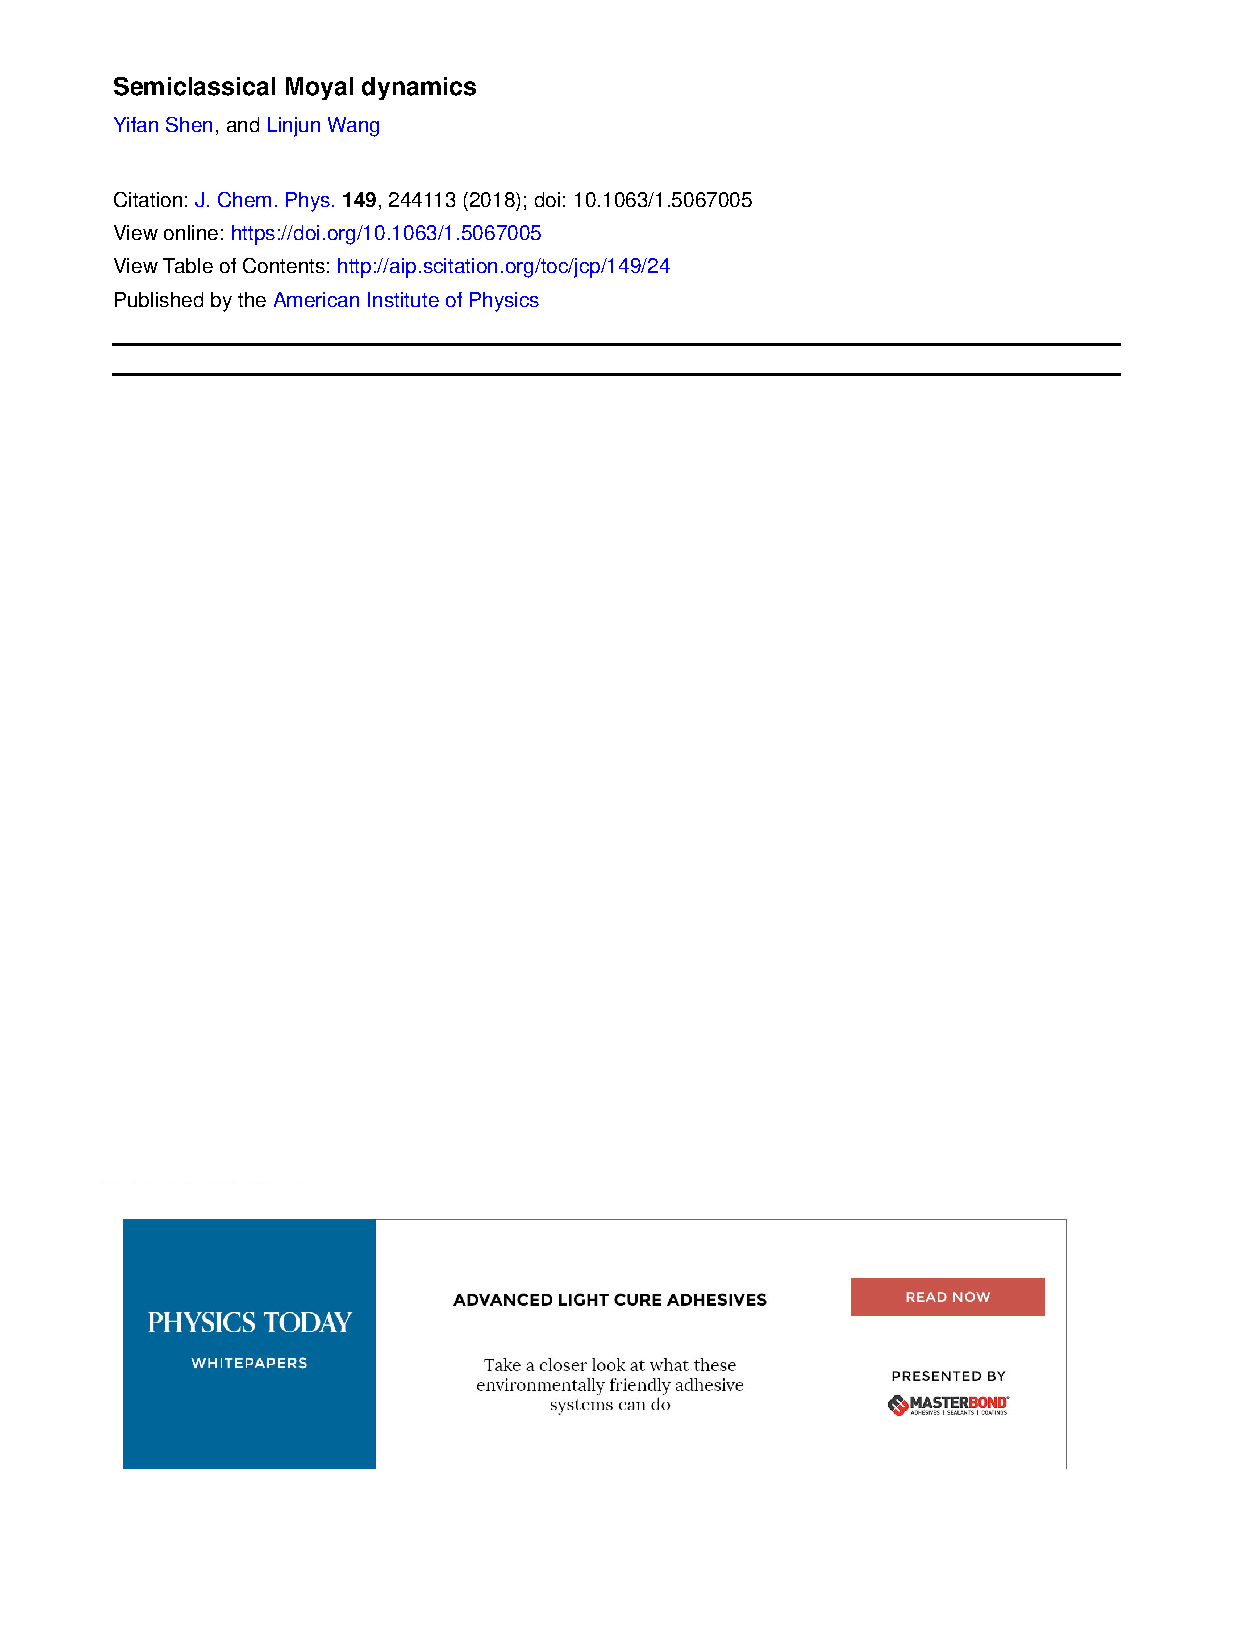
\includepdf[
        pages=1-9,
        scale=0.8,
        pagecommand={\pagestyle{fancy}}
        %frame % remove this line if you don't want outer fram of pdf
    ]{original.pdf}
\end{center}


\end{document}